\documentclass{beamer}
\usepackage[utf8x]{inputenc}
\usepackage{hyperref}
\usepackage[footheight=1em]{beamerthemeboxes}
\usepackage{listings}
\usepackage{color}
%\usepackage{pgfpages}
%\setbeameroption{show notes on second screen=left}
\usetheme{Singapore}

%\usetheme{Frankfurt}


%\addfootboxtemplate{\color{white}}{\color{gray}
  %\insertframenumber/\inserttotalframenumber\null}



\setbeamertemplate{background canvas}{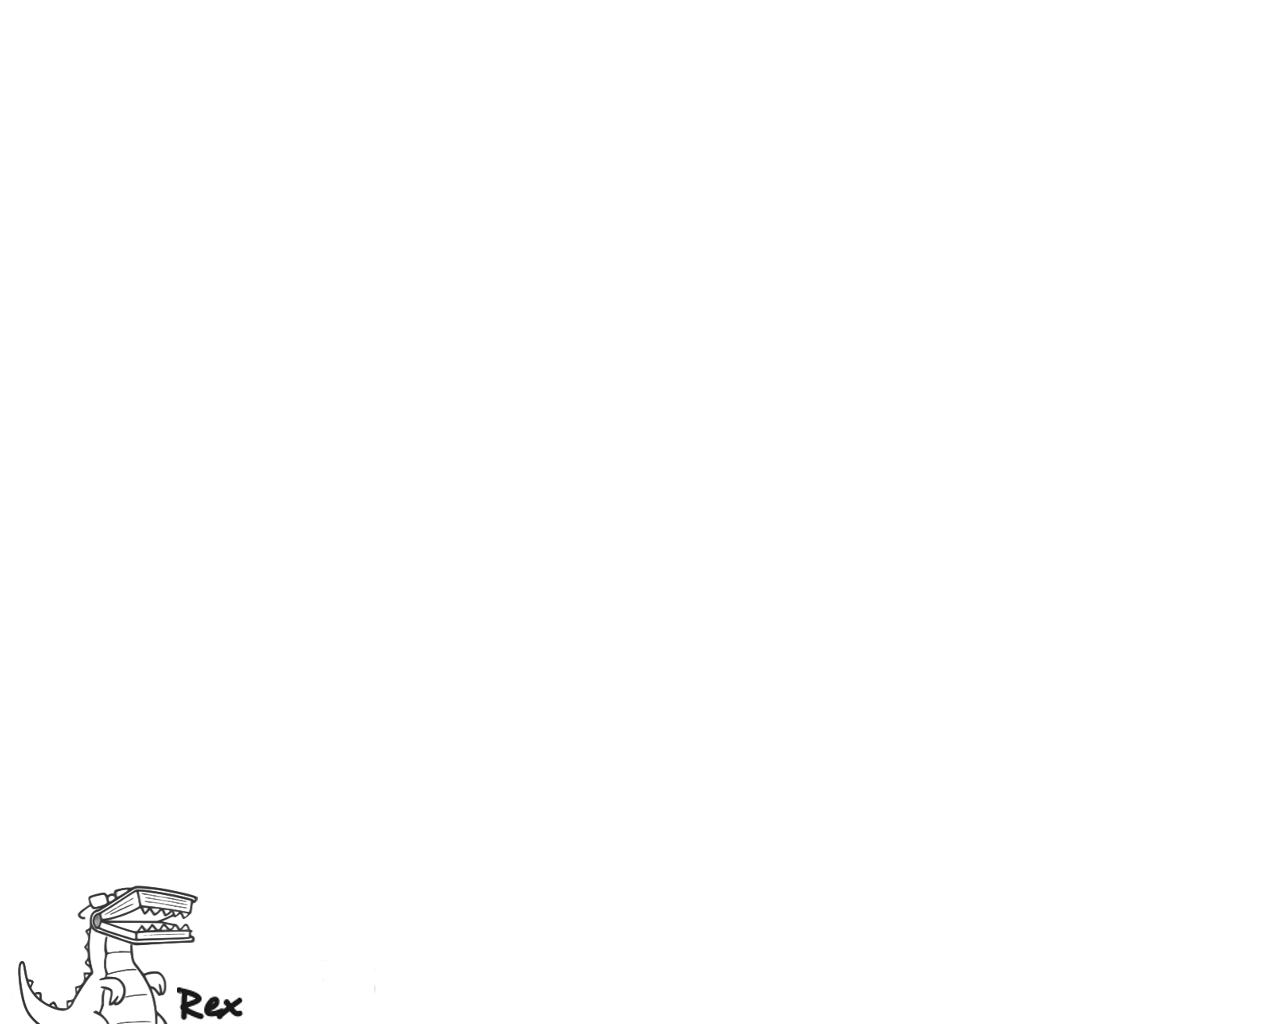
\includegraphics
   [width=\paperwidth,height=\paperheight]{files/fond.png}}


\title{Thésaurus Rex}
\author{Baptiste \textsc{Le-Bail} \and Thibaut \textsc{Marmin} \\ Namrata \textsc{Patel} \and Clément \textsc{Sipieter} \\ Steeve \textsc{Tuvée}}
\institute{Projet BDD GMIN103 : réalisation d'un Thésaurus\\\texttt{https://github.com/marminthibaut/bdd\_projet/}}
\date{20 Janvier 2012}

\begin{document}

% Def variable coloration code source
\definecolor{keyword}{rgb}{0.55,0,0} 
\definecolor{type}{rgb}{0,0.55,0} 
\definecolor{comment}{rgb}{0.7,0.7,0.7} 

\lstset{
basicstyle=\footnotesize\sffamily,
numbers=none,
numberstyle=\footnotesize\color{comment},
keywordstyle=\color{keyword}\bfseries,
commentstyle=\color{comment},
breaklines=true,
fontadjust=true,
columns=fullflexible,
morekeywords=true
}

\AtBeginSection[]
{
  \begin{frame}{Thésaurus Rex}
  \begin{columns}[t]
  \begin{column}{5cm}
  \tableofcontents[sections={1-3},currentsection,hideothersubsections]
  \end{column}
  \begin{column}{5cm}
  \tableofcontents[sections={4-6},currentsection,hideothersubsections]
  \end{column}
  \end{columns}
  \end{frame}
}

\begin{frame}
\titlepage
\end{frame}

\begin{frame}{Thésaurus Rex}
    

  \begin{columns}[t]
  \begin{column}{5cm}
  \tableofcontents[sections={1-3},hideallsubsections]
  \end{column}
  \begin{column}{5cm}
  \tableofcontents[sections={4-6},hideallsubsections]
  \end{column}
  \end{columns}

\end{frame}

\section{Besoins}
\subsection{Fonctionnalités}
\begin{frame}{Fonctionnalités}{Diagramme de cas d'utilisations}
\begin{center}
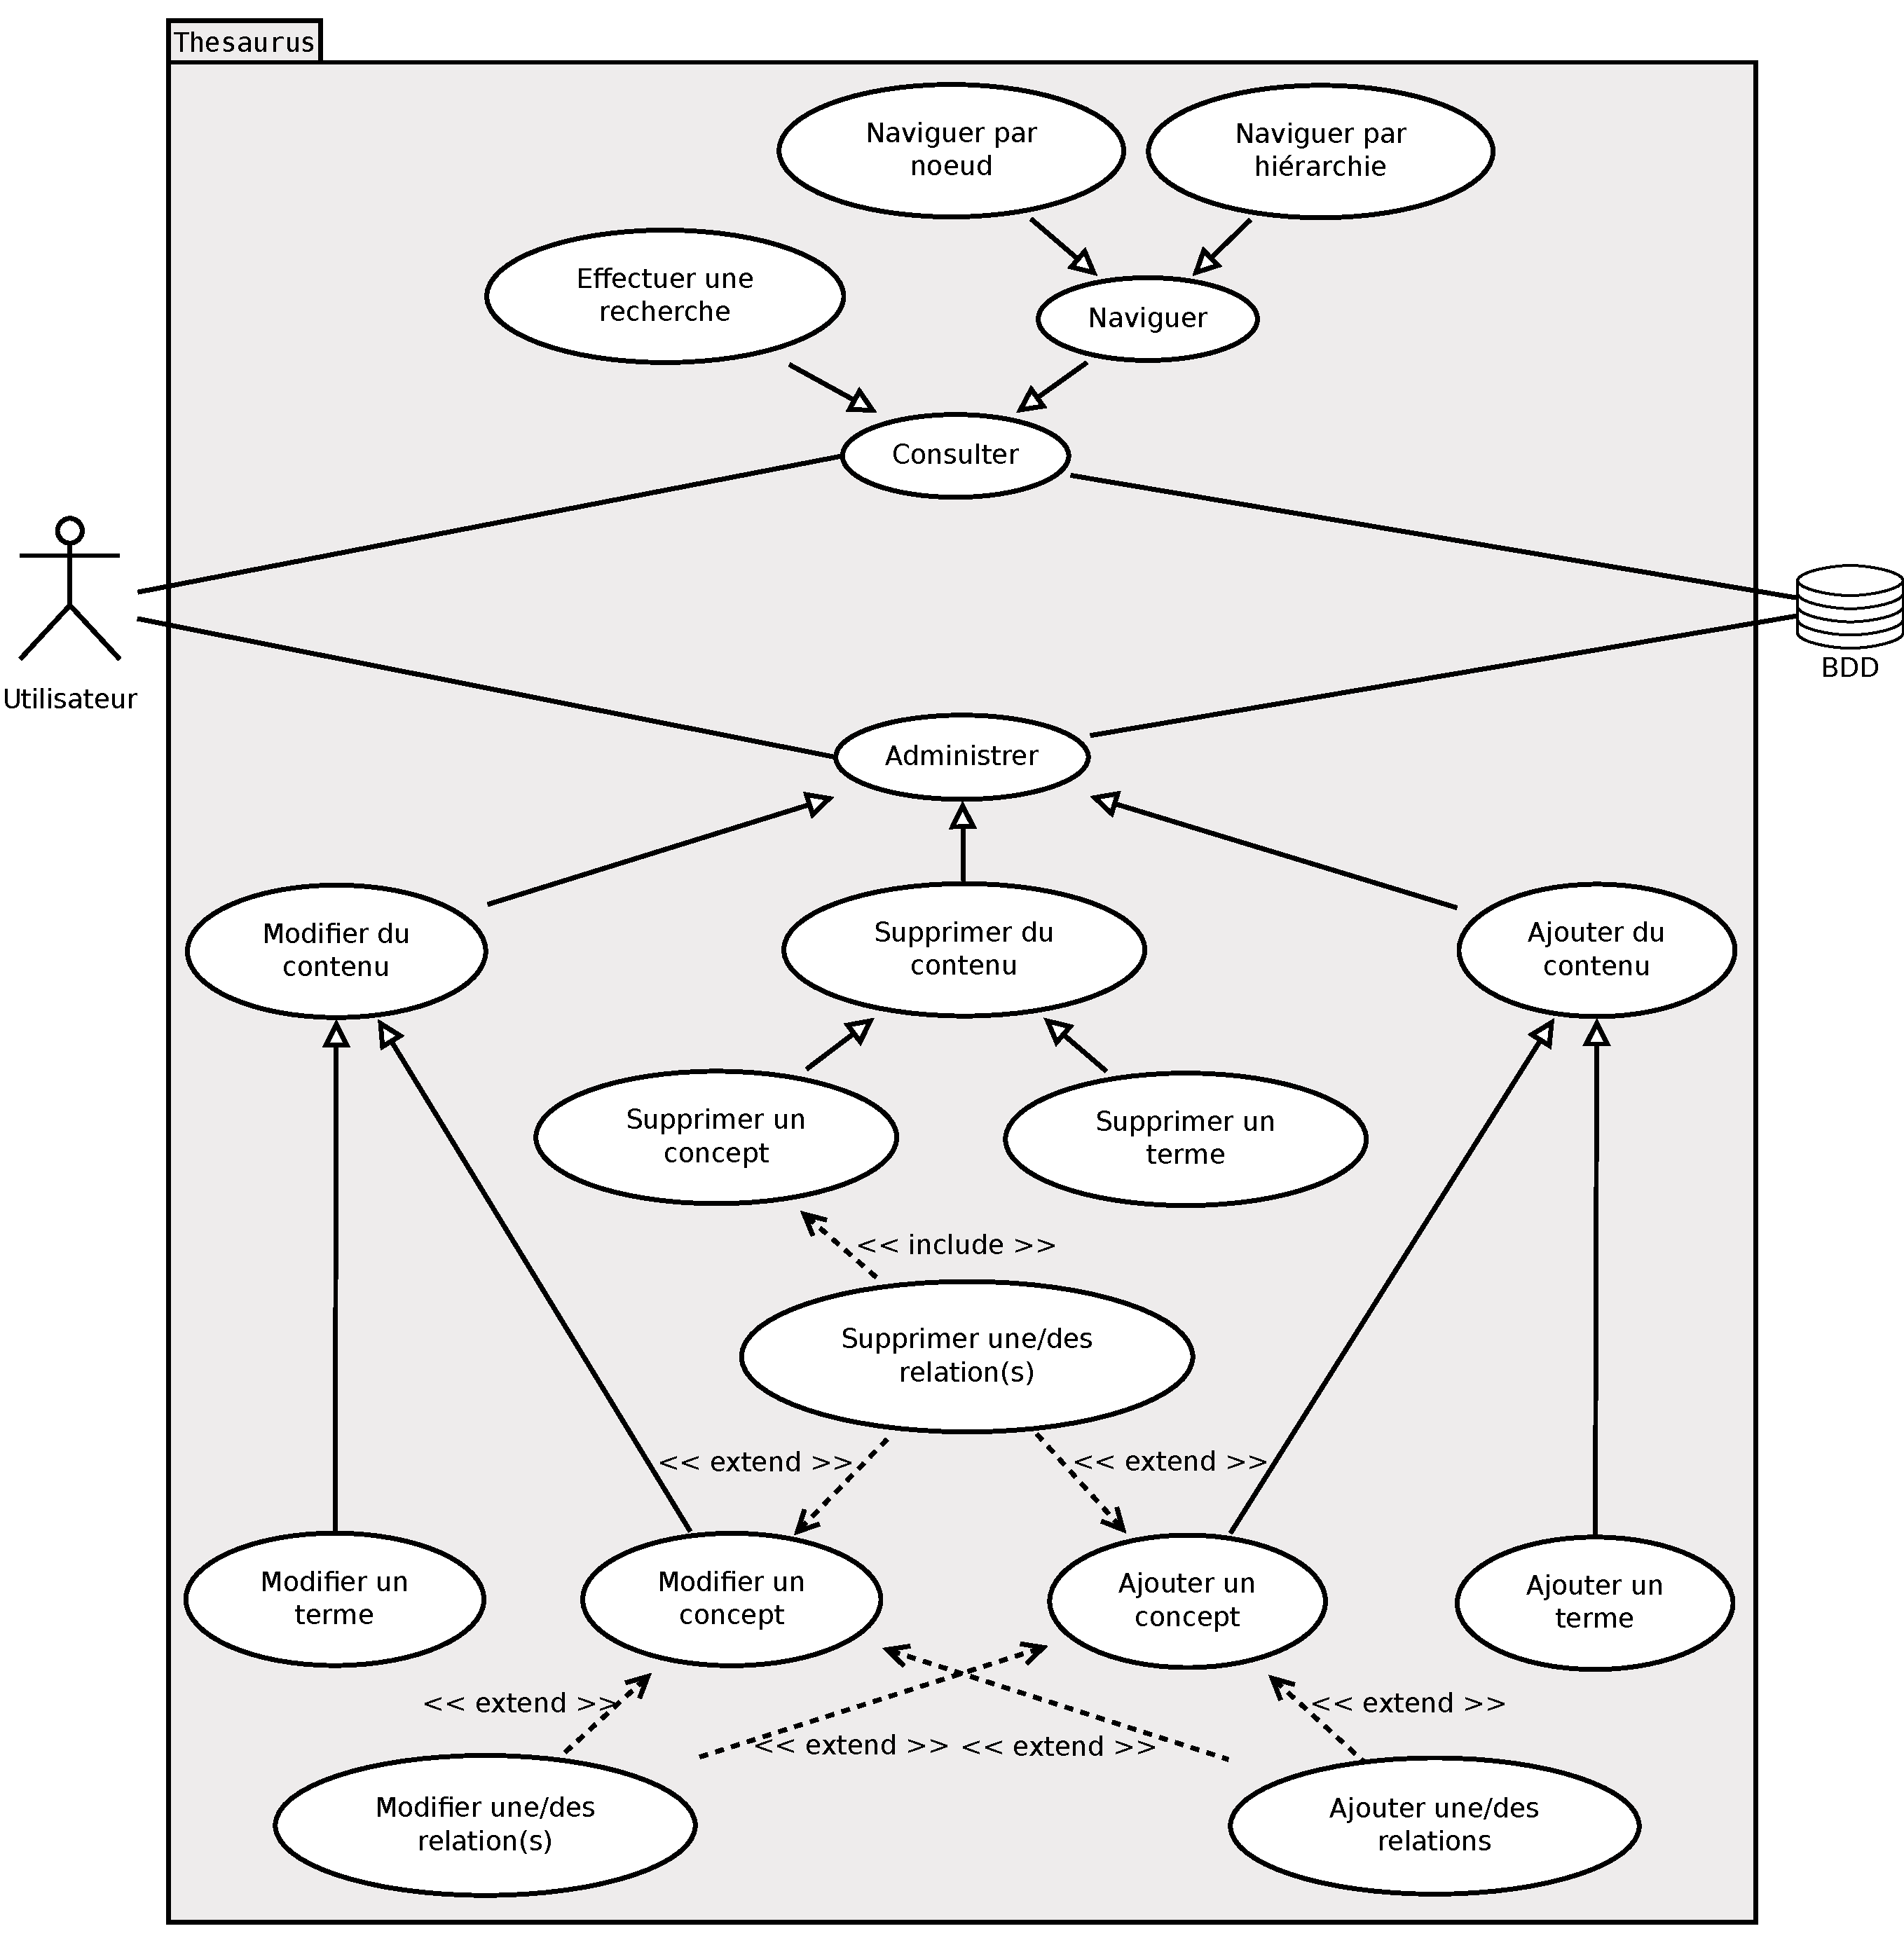
\includegraphics[width=0.65\textwidth]{files/usecase}
\end{center}
\end{frame}

\section{Modélisation}
\begin{frame}{Modélisation}
	Deux type d'entités :
	\begin{itemize}
	\item Termes
	\item Concepts
	\end{itemize}
\end{frame}

\subsection{Une première piste}
\begin{frame}{Une première piste}{Diagramme de classes}
\begin{center}
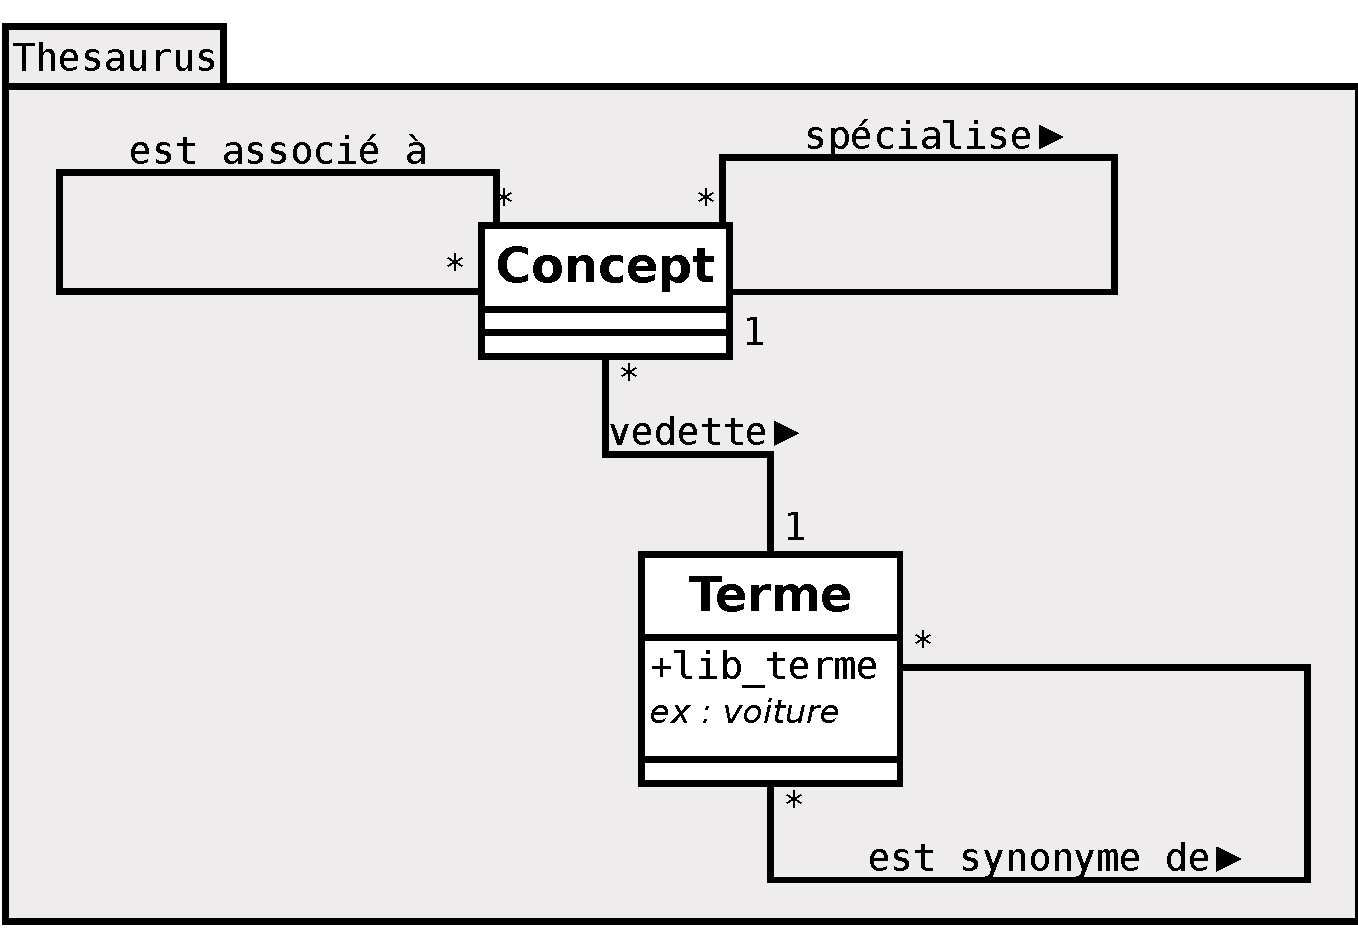
\includegraphics[width=0.5\textwidth]{files/class_v1}
\end{center}
\end{frame}

\subsection{Évolution}
\begin{frame}{Évolution}{Diagramme de classes}
\begin{center}
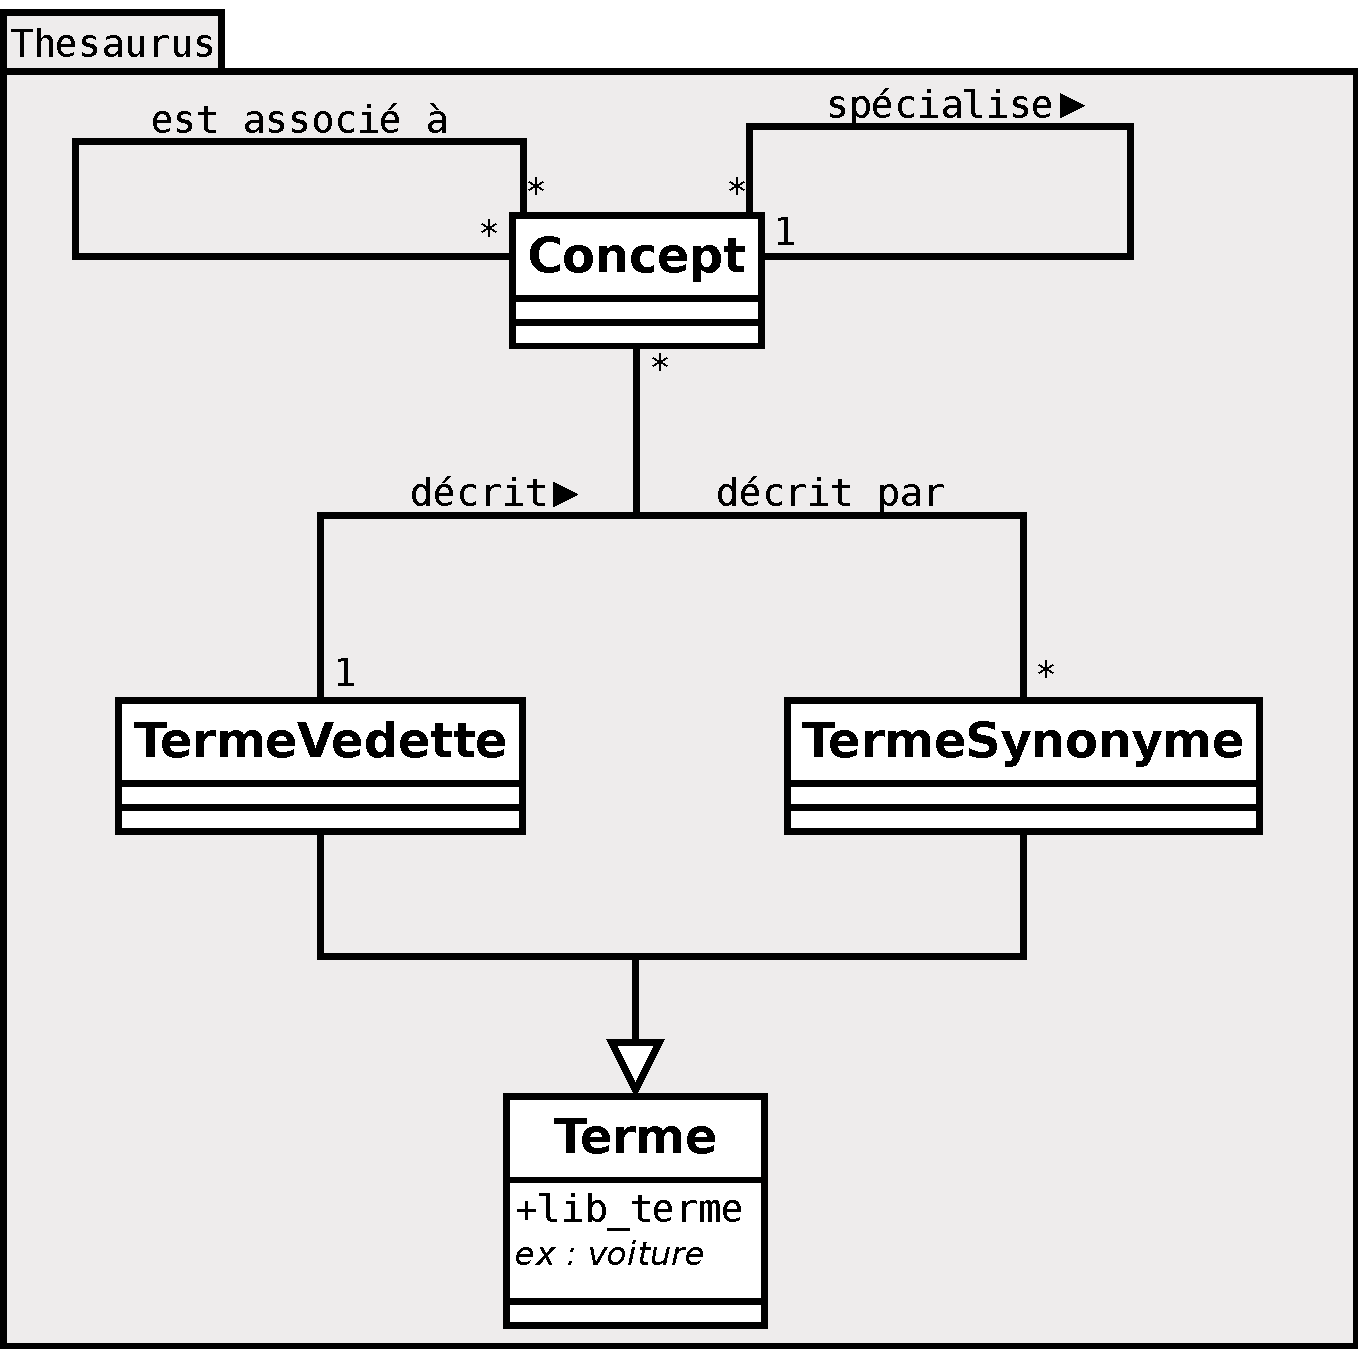
\includegraphics[width=0.5\textwidth]{files/class_v2}
\end{center}
\end{frame}

\subsection{Décision finale}
\begin{frame}{Décision finale}{Diagramme de classes}
\begin{center}
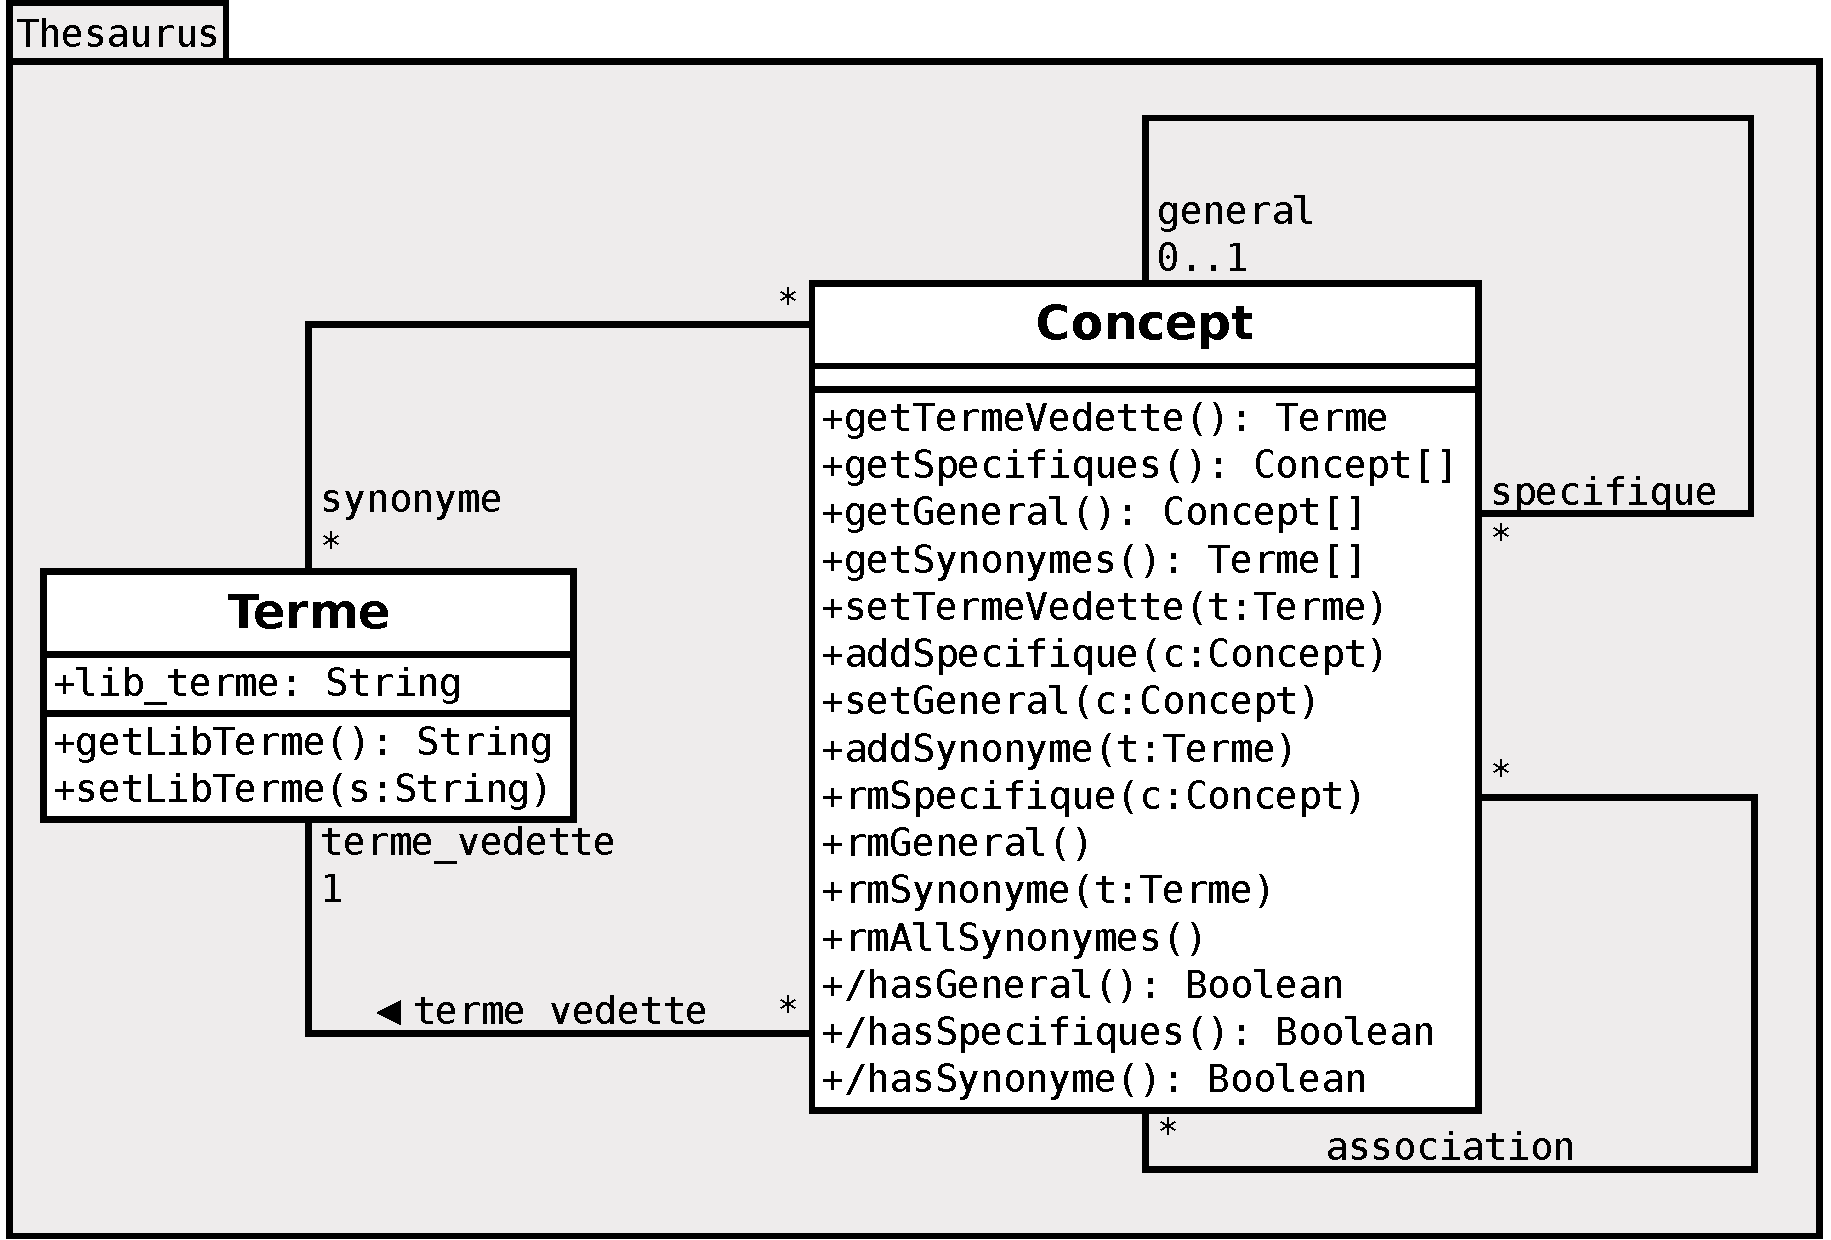
\includegraphics[width=0.6\textwidth]{files/class_v3}
\end{center}
\end{frame}


\section{Choix de conception}
\subsection{Paradigmes}
\begin{frame}{Paradigmes}{Vision objet}
  \begin{block}{Avantages}
    \begin{itemize}
      \item abstraction
      \item réutilisation
      \item maintenance
    \end{itemize}
  \end{block}
  \begin{block}{Inconvénients}
    \begin{itemize}
      \item peu de SGBDO (O2, db4o, ObjectStore)
    \end{itemize}
  \end{block}
\end{frame}

\begin{frame}{Paradigmes}{Vision objet-relationnel}
  \begin{block}{Avantages}
    \begin{itemize}
      \item norme SQL3
      \item accès direct par pointeurs
    \end{itemize}
  \end{block}
  \begin{block}{Inconvénients}
    \begin{itemize}
      \item peu implémenté par les SGBD
      \item différences entre la norme et les implémentations
      \item manque de généricité
    \end{itemize}
  \end{block}
\end{frame}

\begin{frame}{Paradigmes}{Vision relationnel pur}
  \begin{block}{Avantages}
    \begin{itemize}
      \item mature
      \item performant
      \item généricité
    \end{itemize}
  \end{block}
  \begin{block}{Inconvénients}
    \begin{itemize}
      \item schéma relationnel à adapter à une programmation souvent objet
    \end{itemize}
  \end{block}
\end{frame}

\subsection{ORM}
\begin{frame}{ORM}{Qu'est ce qu'un ORM ?}
  \begin{block}{Object relational-mapping}
    \begin{itemize}
      \item composant logiciel
      \item interface entre application objet et BD relationnel
      \item illusion d'une BD objet
    \end{itemize}
  \end{block}
\end{frame}

\begin{frame}{ORM}{Pourquoi ?}
  \begin{itemize}
    \item schéma de données unique
    \item abstraction du SGBD
    \item automatisation de la persistance des données
  \end{itemize}
\end{frame}

\subsection{Décision}
\begin{frame}{Décision}
  \begin{block}{PostgreSQL}
    \begin{itemize}
      \item découvrir un autre SGBD
      \item travailler avec un logiciel libre
      \item respect des standards SQL
    \end{itemize}
  \end{block}
  \begin{block}{ORM}
    \begin{itemize}
      \item avantage d'un schéma objet
      \item avantage d'une base de données relationnelle
      \item découverte d'un ORM
    \end{itemize}
  \end{block}
\end{frame}


\section{Implémentation}
\subsection{Framework}
\begin{frame}{Framework}{Symfony2}
bla bla bla
\end{frame}

\begin{frame}{Framework}{Structure des applications}
bla bla bla
\end{frame}

\begin{frame}{Framework}{ORM Doctrine2}
bla bla bla
\end{frame}

\subsection{Structure de l'application}
\begin{frame}{Structure}{Entités}
Terme et concept
\end{frame}

\begin{frame}{Structure}{Schéma relationnel généré}
\end{frame}

\subsection{Templates finaux}
\begin{frame}{Templates finaux}{Accueil}
\end{frame}
\begin{frame}{Templates finaux}{Formulaire ajout}
\end{frame}
\begin{frame}{Templates finaux}{bla bla bla}
\end{frame}
\begin{frame}{Templates finaux}{bla bla}
\end{frame}

\section{Conclusion \& Démonstration}
\begin{frame}{Conclusion \& Démonstration}
\end{frame}

\end{document}